\chapter{Foundations}
This project is fundamentally about combining existing technologies. In particular, the two most important ones are MicroPsi 2, the most ambitious framework aiming to implement the ideas of the Psi theory, and Minecraft, the super-popular sandbox-videogame.

To understand how and why they were chosen, a brief history of their creation as well as explanations of their basic ideas and relevant insights to their architecture are what this chapter is about.

    \section{Psi Implementations}
Psi has been implemented by different groups at different times. The first implementations are by Dörner and his associates themselves. They used Pascal and developed it for windows environments. This implementation can still be downloaded and runs on Windows 7 installations, for example.

... psi screenshot ... %TODO insert screenshot

The work on Dörner's team's implementation has not been continued, so Joscha Bach and his associates built new implementations of Psi.

From 2003 to 2009 they built an implementation in Java as a set of plugins for the Eclipse IDE called MicroPsi. It consisted of a graphical editor and a 3D simulation-environment. Aiming at better understandability and to maintain platform independence, MicroPsi has been built ground up again in 2012 --- using more lightweight Python code. What is remarkable about the new implementation called MicroPsi 2 (in the following MicroPsi), is that the graphical interface is completely rendered inside a webbrowser --- using state-of-the-art internet- and webapplication-technologies.~\cite{conf/agi/Bach12}

The MicroPsi user interface is rendered completely inside a web browser and the simulation is deployed as a web application. The webinterface is based upon HTML/Javascript and communication in between the browser and the simulation is managed via JSON remote procedure calls. Many GUI components of Twitter's Bootstrap library and the JavaScript graphics library PaperJS are used.~\cite{conf/agi/Bach12}

Matching the concepts of the Psi Theory, MicroPsi simulates agents as neuro-symbolic spreading activation networks. Agents can be placed and researched in simulation environments or physically embodied as robots.~\cite{conf/agi/Bach12}
        
Even though there have been more complex simulation environments (e.g. 3D-worlds) for previous implementations of Psi-architectures, the relatively new MicroPsi has only two fairly simple ones: a 2D-Island and a map of the public transportation system of Berlin. Instead of building another 3D-world, with this project we set out for something more experimental.

        \subsection{Module Overview / Architecture}
MicroPsi modular structure is fairly easy to understand. At first, one can differentiate between the server component (or the web-interface) and the actual simulation code (called "core").

In a minimal setup MicroPsi runs three threads. One thread for the webserver, one for the world simulation and one for every world-adapter (or agent). If more then one agent or more than one world are launched, they are instantiated as additional threads.

Furthermore, the core consists of a runtime component, a user and configuration manager. The runtime works independently of the server and can also by deployed for commandline interaction or other GUIs. It manages the simulations worlds as well as the agents (node net embodiments) and the world-adapters.~\cite{conf/agi/Bach12}

            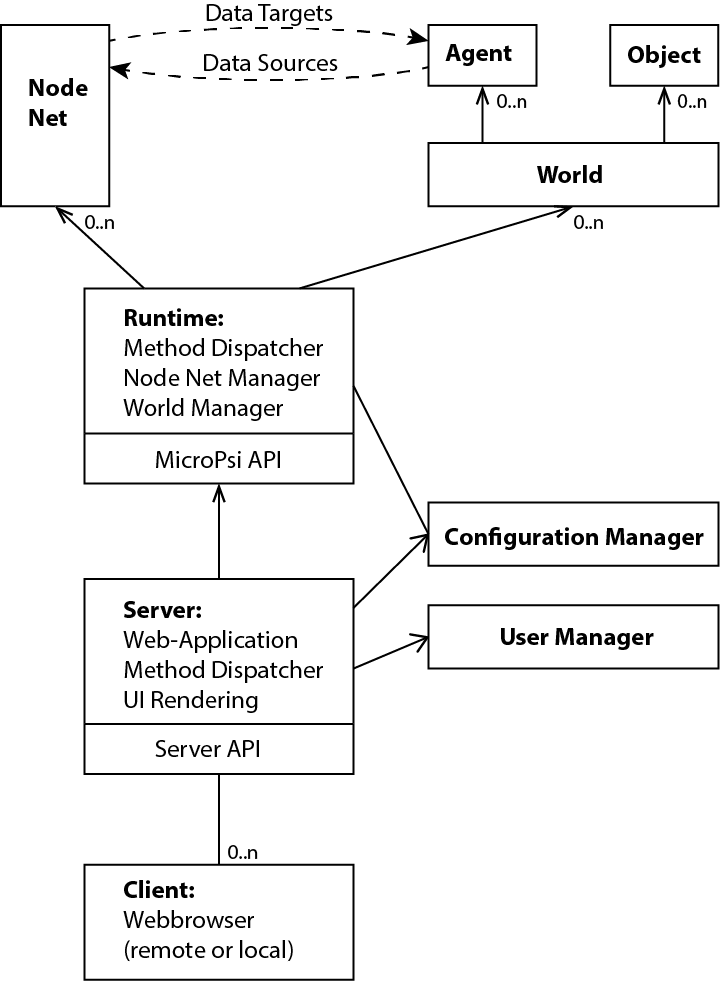
\includegraphics[width=10cm]{graphics/micropsi2_uml}
            
            \subsubsection{Agents}
MicroPsi defines agents as node nets.~\cite{conf/agi/Bach12}
                
"MicroPsi interprets cognitive models as agents, situated in dynamic environments. MicroPsi agents are entirely defined as hierarchical spreading activation networks (SAN), which—for lack of a better name—are called node nets. Node nets are the brains of these agents—or rather, an abstraction of the information processing provid- ed by brains, and the environment provides a body and stuff to interact with.
The body manifests itself as a set of data sources (which can be thought of as the terminals of sensory neurons) and data targets (the abstracted equivalent of motor neurons). By reading activation values from data sources, and sending activation into data targets, the MicroPsi agent may control its body and interact with its world.
MicroPsi’s node nets can be interpreted as neural networks and afford neural learn- ing paradigms. For the purposes of information storage and retrieval, they can be seen as semantic networks with a small set of typed links to express associative, partonom- ic, taxonomic and causal relationships.
Since the nodes can also encapsulate state machines and arbitrary operations over the node net, they can also be understood as components of a concurrent, modularized architecture, with activation spreading as the primary means of communication be- tween the modules."~\cite{conf/agi/Bach12}

            \subsubsection{Environment}
The simulations worlds are the environments in which we can study our node nets behavior. Worlds need to provide the worldadapter --- the interface in between the node net and the simulation. Data sources and data targets have to be defined, to get a functional and meaningful experiment going.~\cite{conf/agi/Bach12}
                
"Within the MicroPsi framework, agents may be embedded into an environment (world). The environment must provide a world adapter wa for each MicroPsi agent. The world adapter offers data sources, from which the agent’s node net may read environmental information, and data targets, which allow the agent to effect changes in the world. Since the environment only has write access to data sources, and read access to data targets, node net and environment may be updated asynchronously.
The world adapter may interface a local multi-agent simulation, a robotic body, a computer game client or simulation server, dynamically updated stock data, etc."~\cite{conf/agi/Bach12}

            \subsubsection{Applications}
At the time of the development of the original development of the framework, the priorized application was building a framework for knowledge representation.~\cite{conf/agi/Bach12}

"Compared with the original implementation of MicroPsi, the current iteration of the framework is still fragmentary; at the time of writing, it supports only a simple generic simulation world for multi agent experiments (instead of the various simula- tion environments provided in MicroPsi 1). Also, 3D viewing components for envi- ronments and facial expressions are completely absent.
The current priority of MicroPsi 2 lies on affective simulation for problem solving experiments (see Bach 2012b), and its application as a general framework for knowledge representation in a hierarchical semantic network."~\cite{conf/agi/Bach12}


            \subsubsection{Core}
Then, there are nodenets. Nodenets can be stored and edited graphically from within the web-interface.

World-adapters are, what makes nodenets and worlds interact with each other. Therefore they provide Data-Sources and Data-targets, which embody the nodenets input from the world (it's senses/sensors) and output (it's muscles?/motors/actuators).

... the core runs the heart of the simulation ...

            \subsubsection{Server}
The server is built on the Python webframework Bottle.~\cite{conf/agi/Bach12}
... the server provides the interface ...

            \subsubsection{Simulation Environments}
... so far, there are an "Island" and an "Berlin" worlds ...

    \section{A! Minecraft}
... a more complex simulation environment could be fun ...

... the story of Minecraft ...
... Minecrafts popularity (and demographics) ...

The story of Minecraft has many interesting sides, but one kind it is without doubt: a story of success.

When Markus ("Notch") Persson built and released the first public version of Minecraft it soon became clear that his creation resonated with many people. The simple concept of world entirely build of standard sized building blocks which the player is allowed to create, destroy and relocate one-by-one let many gamers employ their creativity, explore the Minecraft world and test out it's possibilities and boundaries.

One computer-game in particular stood out in the last years --- not for A.I. reasons though. It is called Minecraft and is benefiting of high popularity ever since its first release in 2009. Since copies of the game can be obtained commercially for the first time in 2011, the different versions of the game sold more than 26 million times - the PC version priced at about 20 Euros. It should be noted, that the games developer studio Mojang is a so called "Indie" developer that is not associated with any classical game publisher but distributes copies of their game exclusively via their own website.

Even though the game can be downloaded and played as a single packet of software, many scenarios of playing the game consist of running a Minecraft server software as well as one client per player. It is possible to mimic the official client by implementing the reverse-engineered Client-Server-Protocol and build artificial players that way.

Minecraft is a complex yet easily accessible virtual world. It is constantly developed and new features are added regularly. It is a massive fanbase and a huge community of game-modifications.

Another interesting aspect about Minecraft is the procedural semantic the game world is generated with and. Trees in Minecraft, for example, may share a similar structure that consists of a trunk and branches and leaves spreading out as fractals, but the particular characteristics of each tree are generated randomly. This makes a Minecraft world somewhat more realistic than most other videogames.

        \subsection{What is a Minecraft world?}
In this section some of the basic concepts (in regards to our A.I. interface) of the game are described. Minecraft worlds are build out of blocks~(see figure ~\ref{mc_block}). Blocks are cubes. There are different kinds (materials) of blocks and they have a single size, which converts to the basic distance unit of Minecraft. One unit can roughly be thought of as equaling one meter.

\begin{figure}[h]
  \centering
    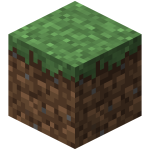
\includegraphics[width=1cm]{graphics/block}
  \caption{A "grass" Minecraft Block}
  \label{mc_block}
\end{figure}
        
A chunk~(see figure ~\ref{mc_chunk}) is a segment of the Minecraft world that is 16 blocks long, 16 blocks wide and 256 blocks high (or deep).~\cite{mcwiki_chunks}

\begin{figure}[h]
  \centering
    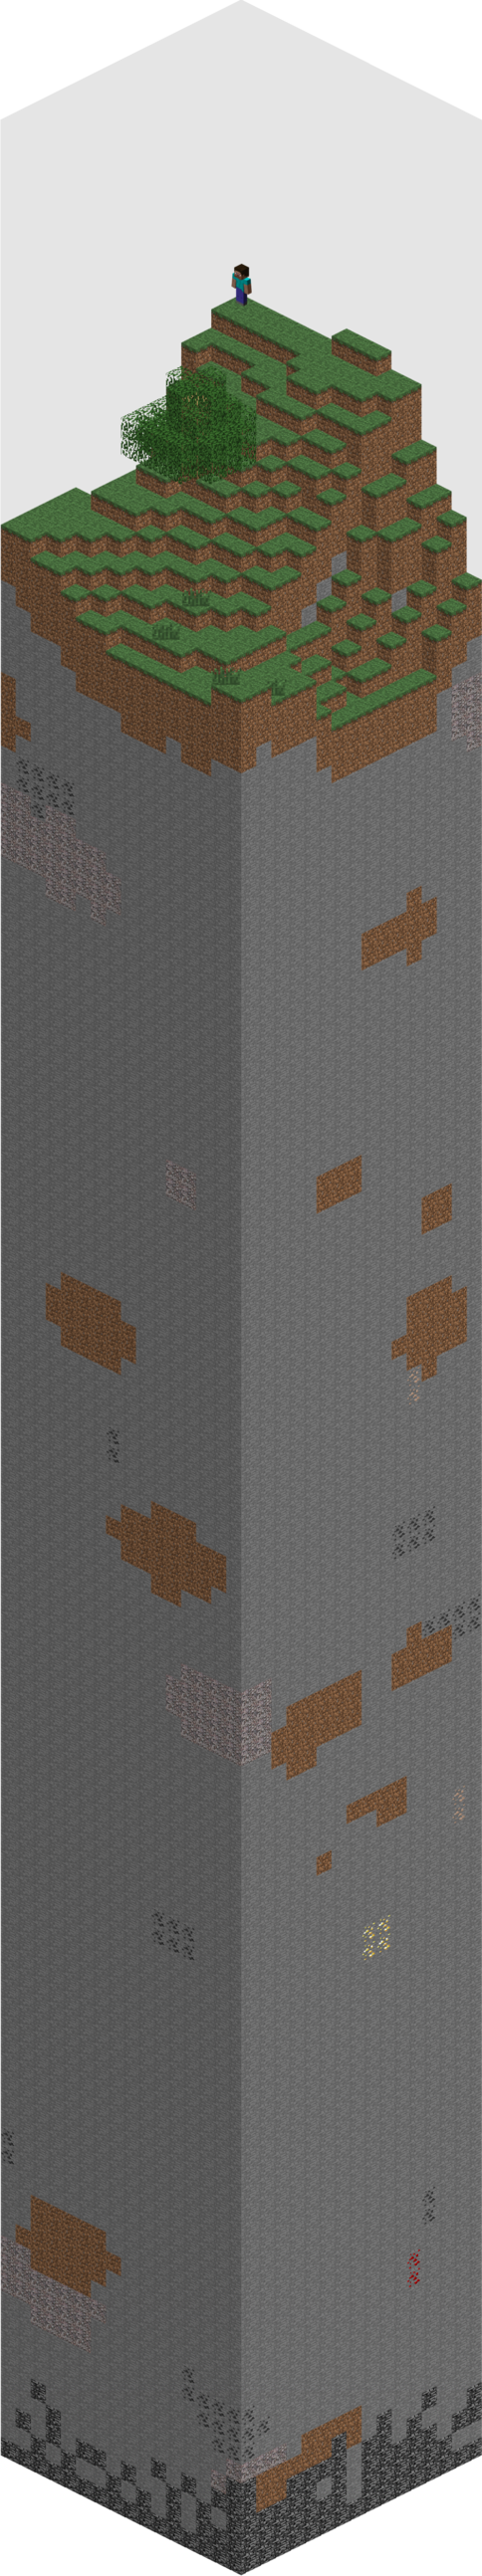
\includegraphics[width=1cm]{graphics/chunk}
  \caption{A chunk}
  \label{mc_chunk}
\end{figure}

"The player"~(see figure ~\ref{mc_player}) is what the playable game-character in Minecraft is called. Usually it is displayed as a humanoid.

\begin{figure}[h]
  \centering
    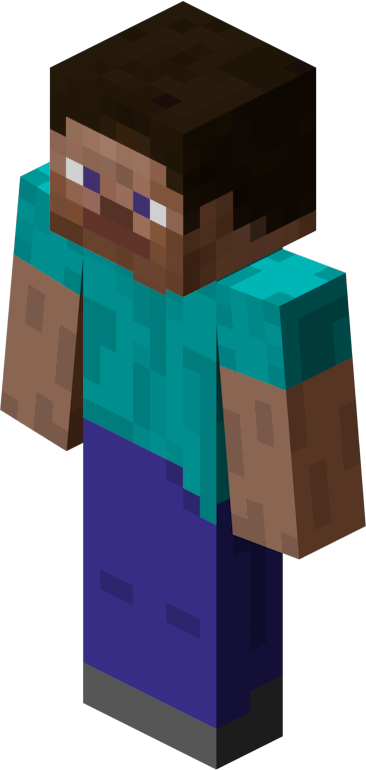
\includegraphics[width=1cm]{graphics/player}
  \caption{"the player" (CC-BY-3.0 Mojang AB) \cite{image_mob}}
  \label{mc_player}
\end{figure}

... brief description of the basic mechanisms (eg. building, mining, crafting) ...
... the game has no predefined "goal" ... other than monsters trying to kill you at night ...

        \subsection{The Client Server Protocol}
Minecrafts Client-Server-Protocol is (at least not to the public) documented by the developer themselves. However, the modding-community found it's ways to gather full knowledge of its structure (probably by using reverse engineering techniques). The protocol is based on packets. 

"All packets begin with a single "Packet ID" byte. Listed packet size includes this byte. Packets are either "server to client", "client to server", or "Two-Way" (both). Packets are not prefixed with their length. For variable length packets, you must parse it completely to determine its length." 

To give an example of one of the easier packets, the "Client Position"-Packet is fairly straight forward. It is exclusively send form clients to servers and starts with the Packet ID (as every Packet does), followed by the X- and Y-coordinates as doubles, the stance value as a double, which is used to to "modify the players bounding box when going up stairs, crouching, etc…", another double for the Z-coordinate and eventually a boolean that describes if the player is on the ground or not.~\cite{protocol}

Knowledge of this datastructure is already sufficient to move around in the Minecraft world. To go forward, one has to figure out the players current position, calculate the absolute coordinates of the destination of the movement in regard of it and send a "Client Position" packet with these coordinates to the server. If the destination is not more than 100 blocks away from the origin, the server accepts the packet. In the official Minecraft client, a players movement from one point to the other is rendered with a smooth transition.

Other than movement, there are defined packets(-structures) for every aspect of the game. May it be the initial handshake, the creation or destruction of blocks or activity of other player- or non-player-characters

... the language an external client needs to speak, to take place in a Minecraft world ...

        \subsection{Suitability of Minecraft as a simulation environment}
There are a number of reasons why using Minecraft as a simulation environment could be useful and lead to interesting results.

First, the game itself is easily accessible. It is developed using Java (for both the client and the server software) and therefore somewhat platform independent. The "desktop computer version" is sold for Windows, Mac OS X and Linux devices. There are official ports to Android, iOS, Xbox 360, the Raspberry Pi an a version for the upcoming "Xbox One" is announced. The desktop versions are priced at 19.95 euros  which makes it affordable to a large audience.
%TODO find out how to typeset €

The game itself already has an enormous audience. It is (like most videogames) especially popular with teenagers (or upcoming scientists). Minecraft being loved by so many people could benefit this project as for giving it more attention.

The game's developer has proven many times (proof?) that it acts very friendly to other developers when it comes to building game modifications and creating content that uses and/or changes original Minecraft content. In other words: They are not at all restrictive, when it comes to user people doing all kinds of things with their creations. This led to the availability of a fairly complete community-sourced  documentation and explanation of virtually every aspect of the game --- including it's software architecture, data structure and protocols. This is useful for this project, as chances are low that they will have anything against this project in the foreseeable future. (In fact, the game's A.I. creator Jon Kagström seems to be fond of this project)

The Minecraft world with it's logic, semantic and functions offers possibilities for an A.I. to proof being able to interact with the environment both on very simple and primitive ways (e.g. moving around) as well as increasingly complex tasks like building, collecting resources, craft items from blocks and interacting appropriately with both well-disposed and hostile other incarnations. %TODO find a better word)
%TODO explain crafting

The semantics of the gameworld share characteristics with the real world. Moving through the world one quickly realizes that it is build up out of different biomes (eg. forest or tundra). Also trees, rivers, mountains and ore veins are not hardcoded but generated procedurally and their structure appears to be (somewhat) fractal.
        
... cheap licenses ...
... developer friendly community and game-studio ...
... sandbox game with many possibilities but no pre-defined goals ...
... procedural semantic ...

Using Minecraft as a simulation environment will give the Psi agent possibilities to show off what kind of sophisticated behavior it is capable of.
... a more complex simulation environment could be fun ...

    \section{A! Minecraft Bots}
    
        ... other popular Bot projects and game modifications ...
    
        \subsection{A! Overview / What has been there so far?}
There exist many projects , that could be considered minecraft ``bots''. One has to differentiate in between two types. On the one hand there are those, that mimic an entire client software and facilitate communication with the server on the default client software's behalf. On the other hand there are bots which are modifications of the original client (or server) software and usually add non player characters --- like animals and other non-human creatures --- to the game. The code is usually injected through one of the popular "modloaders" (eg. Minecraft Forge).

One example (and probably the most advanced one) for an entire bot framework that replaces the client is Mineflayer.~\cite{github_mineflayer} It has a high-level abstraction of the environment (eg. entity knowledge and tracking) and is written in JavaScript using node.js . However, it has not been used for this project, because a python implementation was aimed for.

Opposed to Mineflayer, an example for a game modification bot are the "Cubebots" --- fan-made cubes that aim to help Minecraft players with mundane tasks.\cite{mcforums_cubebots}

... Minecraft Bots with simple as well as sophisticated AI ...
... MicroPsi 2 with Island and Berlin world ...

        \subsection{Spockbot von Nickelpro}
Developed by Nick Gamberini, spock is an open-source (MIT license) bot framework (and therefore a Minecraft client) written in Python. It has been chosen as an essential part of this project for two reasons: Being written in Python it painlessly integrates in existing MicroPsi code and the absence of dependencies (with on exception) leave the code understandable and easy to deploy.
    
        \subsection{Protocol Implementation in spock}
Inside the bot-framework spock, the protocol is implemented as follows:

There are datastructures, that describe the Minecraft protocol.

\begin{figure}[ht]
			\centering
			\begin{minipage}{11cm}
				\begin{pseudocode}
blocks = {
	0x00: "Air",
	0x01: "Stone",
	0x02: "Grass Block",
	...
					\end{pseudocode}
				\caption{data structure for block types}
				\label{snippet_position-packet}
			\end{minipage}
		\end{figure}
		
		\begin{figure}[ht]
			\centering
			\begin{minipage}{11cm}
				\begin{pseudocode}
names = {
	0x00: "Keep Alive",
	0x01: "Login Request",
	0x02: "Handshake",
	0x03: "Chat Message",
	...
					\end{pseudocode}
				\caption{data structure for packet types}
				\label{snippet_position-packet}
			\end{minipage}
		\end{figure}
		
		\begin{figure}[ht]
			\centering
			\begin{minipage}{11cm}
				\begin{pseudocode}
structs = {
	#Keep-alive
	0x00: ("int", "value"),
	#Login request
	0x01: (
			("int", "entity_id"),
			("string", "level_type"),
			("byte", "game_mode"),
			("byte", "dimension"),
			("byte", "difficulty"),
			("byte", "not_used"),
			("ubyte", "max_players")),
					\end{pseudocode}
				\caption{data structure for the packets structures}
				\label{snippet_position-packet}
			\end{minipage}
		\end{figure}
		
These are used, to parse packets as follows:

		\begin{figure}[ht]
			\centering
			\begin{minipage}{11cm}
				\begin{pseudocode}
	def decode(self, bbuff):
		#Ident
		self.ident = datautils.unpack(bbuff, 'ubyte')
		
		#print hex(self.ident)
		
		#Payload
		for dtype, name in mcdata.structs[self.ident][self.direction]:
			self.data[name] = datautils.unpack(bbuff, dtype)
					\end{pseudocode}
				\caption{function for decoding packets}
				\label{snippet_position-packet}
			\end{minipage}
		\end{figure}

\section{Python Multimedia Libraries and Minecraft Clones}
Minecraft's succes inspired many other projects - including a number of Clones (or Minecraft like games) in a wide variety of programming languages and environments.

Interesting projects include Skycraft~\cite{skycraft}, a Minecraft-like browser game based on WebGL.

        \subsection{"Minecraft" by Michael Fogleman}
A particular project, that has the same name as the original game, that inspired it, is "Minecraft" by Michael Fogleman. It is a simple Minecraft slone in under 600 lines of Python and gained some popularity on reddit~\cite{fogle-reddit} and Hacker News.~\cite{fogle_hn}

It is comparably easy to understang and modify. It is based on the Python multimedia library pyglet ( http://www.pyglet.org/ ) .

